%%%%%%%%%%%%%%%%%%%%%%%%%%%%%%%%%%%%%%%%%%%%%%%%%%%%%%%%%%%%%%%%%%%%%%%%%%%%%%%%
\section{Using the \texttt{gedit} Editor on \texttt{Mogon}}

%%%%%%%%%%%%%%%%%%%%%%%%%%%%%%%%%%%%%%%%%%%%%%%%%%%%%%%%%%%%%%%%%%%%%%%%%%%%%%%%
\begin{frame}
	\frametitle{Outline}
	\begin{columns}[t]
		\begin{column}{.5\textwidth}
			\tableofcontents[sections={1-9},currentsection]
		\end{column}
		\begin{column}{.5\textwidth}
			\tableofcontents[sections={10-18},currentsection]
		\end{column}
	\end{columns}
\end{frame}

%%%%%%%%%%%%%%%%%%%%%%%%%%%%%%%%%%%%%%%%%%%%%%%%%%%%%%%%%%%%%%%%%%%%%%%%%%%%%%%%
\begin{frame}
	\frametitle{What is this about?}
	\begin{question}[Questions]\begin{itemize}
			\item What is an Editor?
			\item How do I select one?
			\item How do I use it?
		\end{itemize}
	\end{question}
	\begin{docs}[Objectives]
		\begin{enumerate}
			\item Explain, why you need an editor?
			\item What is an IDE, what an editor?
			\item Starting and using \texttt{gedit} as a beginner level editor.
		\end{enumerate}
	\end{docs}
\end{frame}

%%%%%%%%%%%%%%%%%%%%%%%%%%%%%%%%%%%%%%%%%%%%%%%%%%%%%%%%%%%%%%%%%%%%%%%%%%%%%%%%
\begin{frame}
  \frametitle{Editor vs. IDEs (Integrated Development Environments)}
  \footnotesize
  \begin{columns}[t]
  	\begin{column}{.5\textwidth}
  	  {\normalsize\textbf Editors:}
  	  \begin{figure}[t]
  		 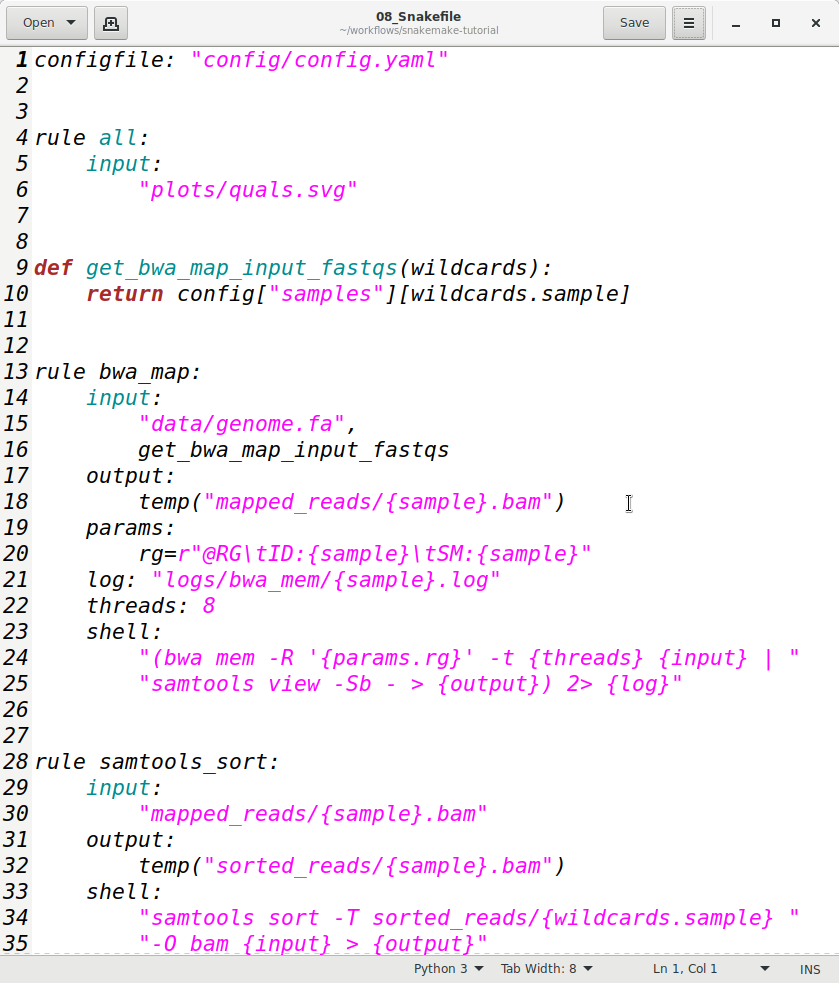
\includegraphics[height=3cm]{editors_and_IDEs/gedit.png}
  		 \caption*{\texttt{gedit} editor as started on Mogon.}
  	  \end{figure}
      \vfill
  	  \begin{itemize}
  	  	\item show syntax highlighting
  	  	\item can edit and save text files
  	  \end{itemize}  
  	\end{column}
  	\begin{column}{.5\textwidth}
  	  {\normalsize\textbf IDEs:}
  	  \begin{figure}[t]
  	  	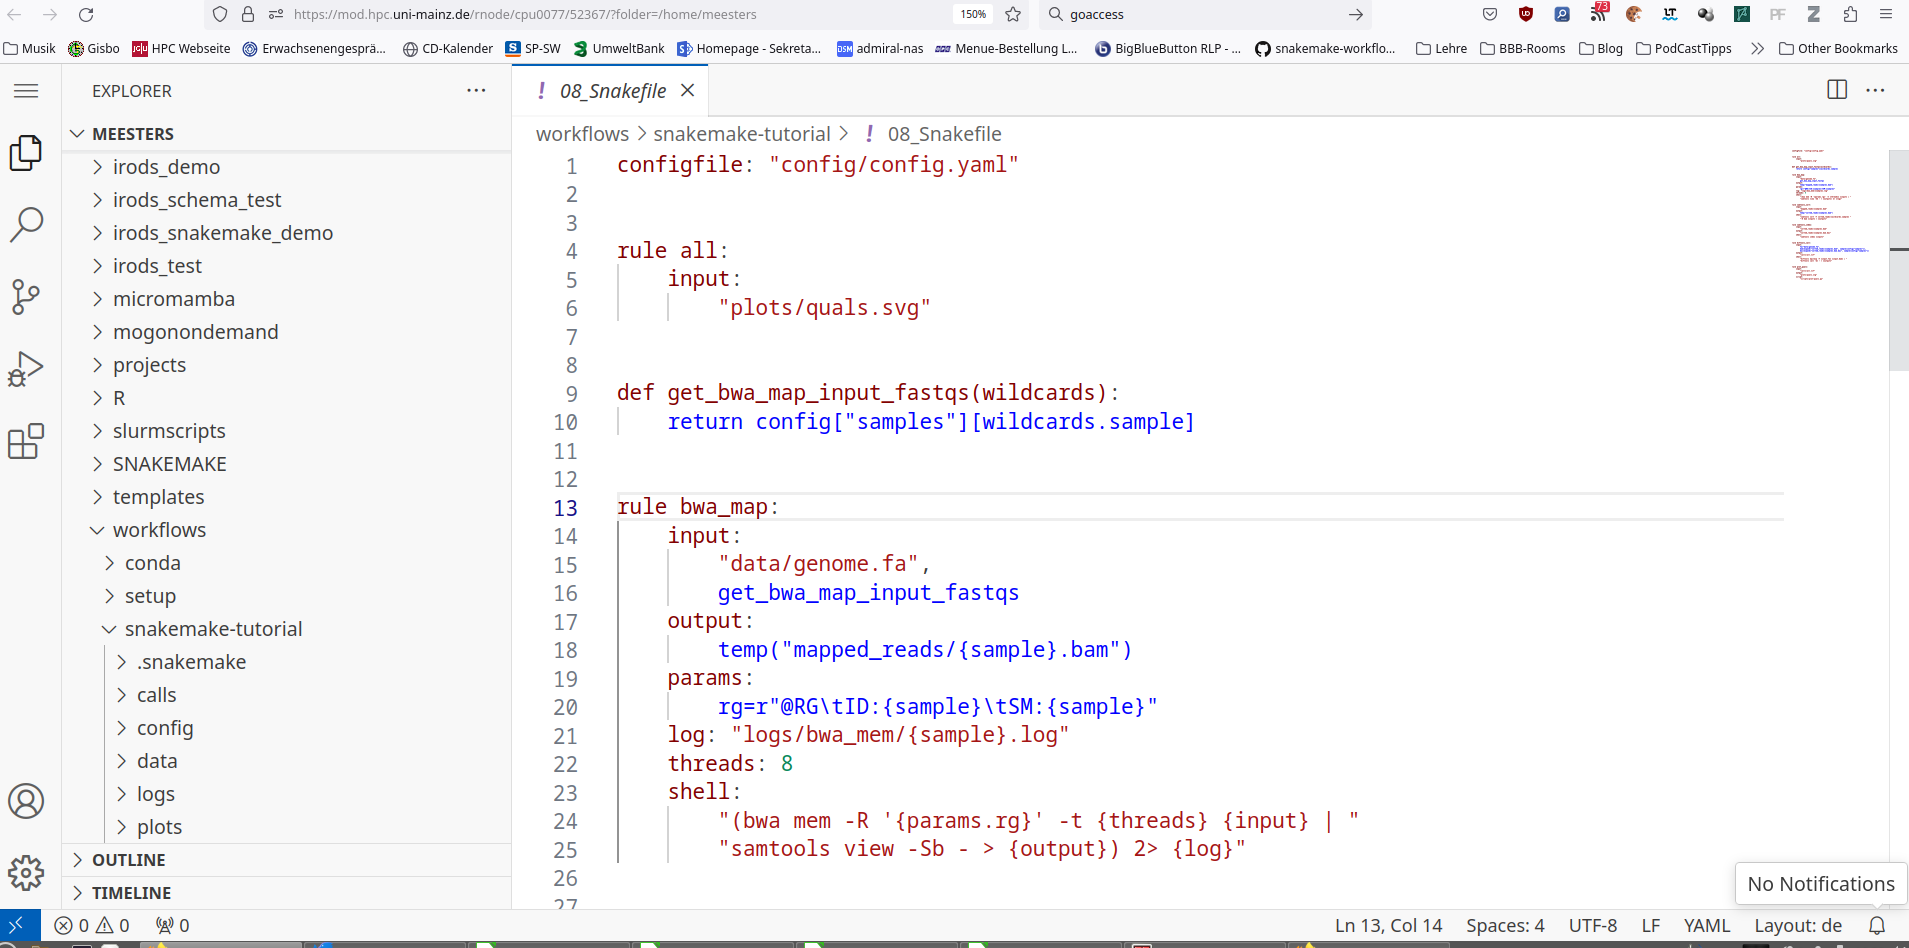
\includegraphics[width=\textwidth]{editors_and_IDEs/MOD_VSC.png}
  		\caption*{\texttt{VSC} as started via MogonOnDemand.}
  	  \end{figure}
      \vfill
      \begin{itemize}
         \item everything an editor can do
         \item handle projects
         \item SCM support
         \item encapsulates environments
         \item \ldots
      \end{itemize}  
  	\end{column}
  \end{columns}
\end{frame}

%%%%%%%%%%%%%%%%%%%%%%%%%%%%%%%%%%%%%%%%%%%%%%%%%%%%%%%%%%%%%%%%%%%%%%%%%%%%%%%%
\begin{frame}<handout:0>
  \frametitle{Which Editor or IDE should I be using?}
  \begin{hint}
     You may use any \emph{any} editor of your liking. These slides introduce \texttt{gedit} as a common denominator.
  \end{hint}
  Rule of thumb:
  \begin{itemize}[<+->]
  	\item start simple, e.\,g. with \texttt{gedit} or \texttt{nano}
  	\item go for an IDE, when the project requires it. Usually projects give recommendations or even requirements.
  \end{itemize}
\end{frame} 

%%%%%%%%%%%%%%%%%%%%%%%%%%%%%%%%%%%%%%%%%%%%%%%%%%%%%%%%%%%%%%%%%%%%%%%%%%%%%%%%
\begin{frame}[fragile]
  \frametitle{Starting \texttt{gedit}}
  \begin{columns}[T]
  	 \begin{column}{.5\textwidth}
  	   \texttt{gedit} is a simple-to-use text editor, very suitable for beginners.\newline
        Start \textit{gedit}:
       \begin{lstlisting}[language=Bash, style=Shell]
$ gedit @&@
$ #or
$ gedit <path to file> @&@
      \end{lstlisting}
      The \altverb{@} starts the process in the background, if you forgot it:
      \begin{lstlisting}[language=Bash, style=Shell]
$ [Ctrl+z]
$ bg
      \end{lstlisting}	
    \end{column}
    \begin{column}{.5\textwidth}
      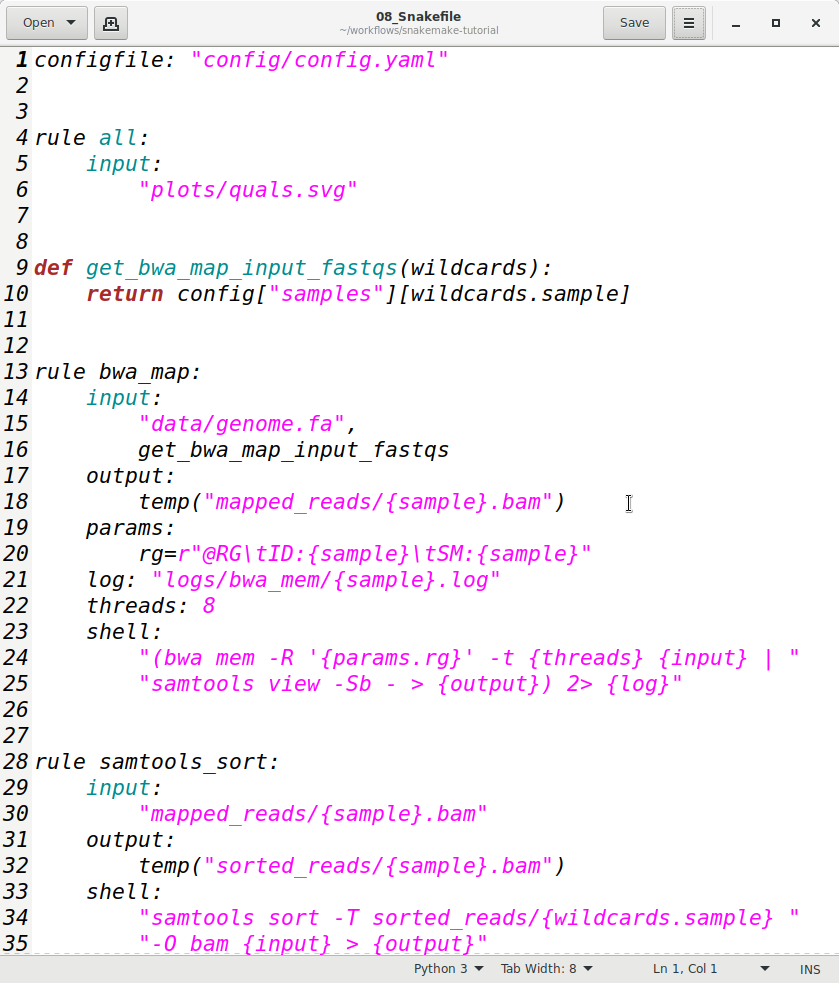
\includegraphics[height=3cm]{editors_and_IDEs/gedit.png}	\newline
      If you want to turn on syntax highlighting for \texttt{Snakefile}s, you have to select \texttt{Python3} as the language. (We will do this, when we hit\texttt{Snakefile}s for the first time.)
    \end{column} 
  \end{columns}
  \begin{hint}[Note]
    We will exercise and show this, when we start coding!
  \end{hint}
\end{frame}